\chapter{Music Generation Models}\label{ch:ch4}
State-of-the-art models in music generation are mostly comprised of ANN models. Some music generation tasks have already seen a Transformer application, while others (such as expressive performance generation) have not. We will provide an overview of the existing state-of-the-art in EMP generation and transformer-based music generation models. We also give some background into the data representation and feature engineering of each model. 

\section{Existing Expressive Musical Performance Generation Models}\label{sec:emp_generation_models}
EMP generation models fit into one of two categories, rule-based and data-based. Rule-based systems use hardcoded rules derived using pre-existing musical knowledge and empirical studies involving human cognition. Data-driven models rely on ML methods and use an existing dataset of human performances as a guide to learn the mapping between score features and performance features. Data-based models most commonly use sequential probabilistic or non-linear ANN methods~\cite{cancino2018computational}, although there has been previous work with linear and non-sequential modeling.~\citet{cancino2018computational} give a complete overview of all relevant EMP generation models. We describe a few models, both rule and data-based, which are pertinent to our work. 

\subsection{Rule-Based EMP Models}
The KTH system~\cite{friberg2006overview} sits at the center of rule-based EMP models and created the foundation for all EMP generation models. Development of the KTH system started in the 1980s and has continued well into the 21st century. The KTH system's initial methodology defined rules relating to musical composition structure and how it affects a resulting performance. The first set of rules applied specifically to singing synthesis and were later adapted to general musical performance. 

Since then, there have been two general methods in the continued development of the KTH rule system. The first is that of \emph{analysis-by-synthesis}, which involved using the rules to synthesize musical performances presented to human listeners (both professional and non-professional), gathering listening feedback, and then using this feedback to modify the rules where needed. The second was an \emph{analysis-by-measurement} method. This method uses direct computation to evaluate a computational generated performance by comparing it with an existing real performance%
\footnote{This evaluation method is consistent with the data-driven approaches but can generally apply to any model. Data-driven models use the performance data to directly build the model, whereas real performance data in the KTH system is for evaluation purposes only. Any further updates to the model still rely on a hardcoded set of rules.}. The \emph{analysis-by-synthesis} and \emph{analysis-by-measurement} correspond to qualitative and quantitative evaluation methods, respectively. Example rules from the KTH system are found in Figure \ref{tab:kth-rules}.


\begin{table}
    \setlength{\extrarowheight}{7pt}
    \begin{center}
    \begin{tabular}{l | l }
        % \hline
        \textbf{Phrasing} & \\
        \hline
        Phrase Arch & Create arch-like tempo and sound level changes over phrases \\
        Final ritardondo & Apply a ritardando in the end of the piece \\
        High Loud & Increase sound level in proportion to height \\
        \textbf{Micro-level timing} & \\
        \hline
        Duration contrast & Shorten relatively short notes and lengthen relatively long notes \\ 
        Faster uphill & Increase tempo in rising pitch sequences \\
        \textbf{Articulation} & \\
        \hline
        Punctuation & Find short melodic fragments and mark them with a final micropause \\
        Score legato/staccato & Articulate legato/staccato when marked in the score \\
        Repitition articulation & Add articulation for repeated notes \\
        Overall articulation & Add articluation for all notes except very short ones 
        % \hline
    \end{tabular}
    \caption{Some of the KTH rules given by~\citet{friberg2006overview}.}
    \label{tab:kth-rules}
    \end{center}
\end{table}

To our knowledge, the KTH rule-based system is the first sophisticated computational model for generating expressive performance. The explicitly defined rules in the KTH system may be those we expect a data-based model to learn.~\citet{widmer2002machine} shows that data-driven methods learn some rules consistent with the KTH rules and some that are not. Model evaluation's problematic nature may describe this phenomenon, as it is not straightforward how to determine which rules are more ``correct'' than others. Nevertheless, the KTH rule system has been an essential milestone in the evolution of EMP generation. 

\subsection{Data-Based EMP Models: Basis Function Models}\label{sec:data-based}
The Basis Function Modeling (BM) framework for EMP describes the complete end-to-end process involving musical performance generation and analysis. This end-to-end process includes mathematical definitions of score and performance features, computational models for EMP, and the data processing necessary to convert MusicxML to input score features and output performance features to MIDI.%
~\citet{eduardo2018computational} outlines the full mathematical definition of the BM framework, the evolution of the framework, and its application with specific feature and model definitions.

\subsubsection{Features}
The name ``Basis Model'' is derived from the BM framework's definition of ``Basis Functions.'' Basis Functions capture different aspects of a score into numerical encodings (i.e., score features). There are some relatively straightforward Basis Functions, such as the duration of notes and MIDI pitch (we described these features as the ``low level'' of the score hierarchy in section \ref{sec:scores}). However, most of the information in a score cannot be represented so easily. It becomes a theory-laden activity to use musical background knowledge to find good score information encodings, especially at the mid and high levels.

% mp for matched performance
\newcommand{\mperf}{\beta_{\Omega}}

The BM framework defines $\Omega$ as a space containing aspects of a score. A score basis function $\varphi: \Omega \rightarrow \mathbb{R}$ will map elements of a score into some numerical expression based on an aspect of the score. The value of a score basis function for one element $x_i \in \Omega$ is denoted as $\varphi (x_i)$. For example, the score basis function for pitch, 
\begin{align*}
\varphi_{pitch} (n_i) = \textrm{MIDI}_{\textrm{pitch}}(n_i)   
\end{align*}
will represent the pitch of a given note as the numerical MIDI pitch. The basis function for dynamic markings, such as forte, would be defined as 
\begin{align*}
\varphi_{\mnot{f}} (n_i) = forte(n_i)   
\end{align*}
where $forte(n_i)$ returns 1 if the score element is marked with $\mnot{f}$, and 0 if it does not. 

Similarly to basis functions, the BM framework defines \emph{expressive parameters} which are mathematical encodings of information taken from a performance matched to a score. An \emph{expressive encoding function} $y: \mperf \rightarrow \mathbb{R}$ will encode an event in a matched performance into an \emph{expressive parameter}, or performance feature. The value of each parameter corresponding to a score element $x_{i} \in \Omega$ given a matched performance $\mperf$ is denoted as $y(x_i \vert \mperf) = t_i$ where $t_i \in \mathbb{R}$. Example encoding functions are 
\begin{align*}
y_{\textrm{dyn}}(n_i \vert \mperf) = \textrm{MIDI}_{\textrm{vel}}(n_i) \textrm{ and } y_{\textrm{tempo}}(n_i \vert \mperf) = \textrm{bpm}(n_i)
\end{align*}
which represent expressive dynamics as MIDI velocity and expressive tempo as a local measure of bpm, respectively. 

There are many possible definitions for both basis and expressive encoding functions. Here we give some example expressive encoding functions which are defined in the first iteration of the BM framework and provide the foundation for feature set we use. Refer to~\citet{eduardo2018computational} for a full list of both basis functions and expressive encoding functions

% \textbf{Basis Functions}

% % pfunc for pitch function
% \newcommand{\pfunc}[1]{\varphi_{\textrm{pitch}}^#1(n_i)}
% \newcommand{\pfuncnorm}{\varphi_{\textrm{pitch}}(n_i)}
% % midip for midi pithc
% \newcommand{\midip}{\textrm{pitch}}
% \begin{itemize}
%     \item \textbf{Polynomial Pitch Model}: This model is presented by~\citet{grachten2012linear} and describes the dependency of expressive dynamics (MIDI velocity) on pitch. This model defines three different pitch functions. 
%     \begin{align*}
%     \pfuncnorm{} = \frac{\midip (n_i)}{127} \quad \pfunc{2} = \left(\frac{\midip(n_i)}{127}\right)^2 \quad \pfunc{3} = \left(\frac{\midip (n_i)}{127}\right)^3    
%     \end{align*}
%     \item \textbf{Dynamics Markings}: These are functions which encode dynamics markings such as \mnot{p}, \mnot{f}, and \mnot{crescendo}. There are three different types of dynamics encoding functions. The first is an impulse function  which is a binary indicator of a dynamic marking for a single note (this applies to single note marking such as an accent \wedge). The second is a ramp function which gradually increases or decreases a value from note to note (useful for \mnot{crescendo} or \mnot{decresenco} markings which apply to a specified number of notes). The last is a constant function which is either on or off for a set of notes at a time (useful for markings such as \mnot{p} or \mnot{f} which apply to a group of notes at a time). Each dynamic function is shown graphically in figure \ref{fig:dynamics_functions}.
%     \item \textbf{Inter-Onset-Interval (IOI)}: This includes a total of six basis functions which include the difference in onset times of a group of notes belonging to a particular note onset $o_i$ an its surrounding note onsets. The IOI is calculated for the onsets between $(i - 2, i-3), (i-1, i-2), (i, i-1), (i, i+1), (i+1, i+2), \textrm{ and } (i+2, i+3)$. These functions provide context for the local tempo structure of the composition. 
%     \item \textbf{Duration}: A basis function that encodes the notated duration of a single note. 
% \end{itemize}

% \begin{figure}
%     \centering
%     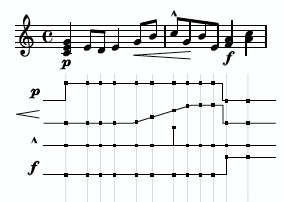
\includegraphics[width=0.7\linewidth]{figs/ch4/dynamics_functions.png}
%     \caption{An illustration of the different dynamics basis functions, taken from~\citet{eduardo2018computational}. The function describing \mnot{p} is a constant function, which is activated for every note until the presence of a different dynamic marking, \mnot{f}. The function describing the crescendo (the second from the top) is a ramp function and gradually increases until the crescendo finishes. The function describing the accent (third from the top) is an impulse function and holds a value of 1 for the note which contains the accent mark. }
%     \label{fig:dynamics_functions}
% \end{figure}

\newcommand{\iois}{\textrm{IOI}_{o(n_i)}^{score}}
\newcommand{\ioip}{\textrm{IOI}_{o(n_i)}^{perf}}
\textbf{Expressive Encoding Functions}
\begin{itemize}
    \item \textbf{MIDI Velocity}: This encoding function uses the recorded hammer-velocities of the performed notes as a proxy for expressive dynamics. The loudness of a note is estimated as a normalized MIDI velocity value. 
    \begin{align*}
    y_{vel}(n_i) = \frac{\textrm{vel}(n_i)}{127}
    \end{align*}
    \item \textbf{log BPR}: The Beat Period Ratio (BPR) is a way to define the local tempo calculated for every note. It uses the Beat Period (BP), defined as 
        \begin{align*}
        BP(n_i) = \frac{\ioip}{\iois}
        \end{align*}
    where $\ioip$ and $\iois$ are the IOI for the performance and score onsets at note $n_i$. The final log BPR is defined as 
        \begin{align*}
        y_{\textrm{log bpr}}(n_i) = log_2\frac{\textrm{BP}(n_i)}{\textrm{BP}_{ave}},
        \end{align*}
    where $\textrm{BP}_{ave}$ is the average BP over the entire piece. This normalizes the local BPR definition according the global tempo of the piece. 
    \item \textbf{Timing (deviation}): Whereas the log BPR defined above encodes the tempo of a performance (how ``fast'' it is being played), the function for timing encodes expressive timing deviations from the indicated timing of a score. It is defined as 
        \begin{align*}
        y_{\textrm{tim}} = \hat{o}^{perf}(n_i) - \textrm{onset}_{perf}(n_i)
        \end{align*}
     where $\hat{o}^{perf}(n_i)$ is an estimation of the ``correct'' onset time, and $\textrm{onset}_{perf}(n_i)$ is the actual observed onset of a note (see section 3.3.1 of~\citet{eduardo2018computational} for a full working example). 
    \item \textbf{log Articulation}: Articulation is a measure of the lengthening or shortening of a performed note duration relative to a noted duration and the current local tempo. The articulation is computed by dividing the measured note duration by the duration given by the score. It is defined as 
        \begin{align*}
        y_{\textrm{log art}}(n_i) = \textrm{log}_2\frac{\textrm{duration}_{perf}(n_i)}{\textrm{duration}(n_i)BP(n_i)}
        \end{align*}
    
\end{itemize}

\subsubsection{Models}
BM framework computational models first started as simple linear non-sequential models that learned the relationship between a set of defined basis functions and a single expressive parameter, such as MIDI velocity. This version of the BM models each expressive parameter independently from all others and implies that one expressive parameter's interpretation will not affect the other. Although this is not necessarily the case in actual performance\footnote{For example, the effect of a \mnot{crescendo} marking may affect both the dynamics and the tempo at the same time.}, it is a simplifying mathematical assumption that makes the models' development and interpretation simpler. Both standard least squares regression and a probabilistic Bayesian approach are used to model the linear relationship. 

The BM framework later introduced non-linear and sequential models, both as ANNs. A standard Feed-Forward Neural Network (FFNN) added the capability for non-linear modeling. This model showed an increase in both the goodness-of-fit and predictive accuracy over the linear model. A standard RNN was used to implement the sequential model with features where the time-dependent and sequential nature of music was relevant. Used in conjunction with a FFNN, this model performed the best relative to all other models.

\newcommand{\vnet}{VirtuosoNet}
\newcommand{\vnetf}{VirtuosoNet framework}

\subsection{Data-Based EMP Models: \vnet{}}
\vnet{}, similarly to the BM framework, is a complete end-to-end system for training EMP models and generating novel performance. Although \vnet{} does not explicitly define a clear mathematical framework and abstract representations of EMP, as does the BM framework, it contains all of the moving parts necessary to train an EMP model from scratch. We make a distinction between \vnet{} as a set of NN-based EMP models and the \vnetf, which comes with all of the necessary data processing and featuring engineering as well as model training. 

\subsubsection{Features}
The \vnetf{} defines both input and output features. Input features contain standard score data such as pitch, timing, key, and metric information. The \vnetf{} uses these features as well as more detailed note level information such as the duration of rests, articulation markings, and others. The framework's output features are similar to those of the BM defined above and include tempo, note onset deviation, MIDI velocity, and articulation. Additionally, the \vnetf{}, unlike any other EMP generation model, uses features to model the pedal directly. They include the pedal value at note onset, pedal value at note offset, minimum pedal value between note onset and note offset, and minimum pedal value between note offset and the next note's onset. A full list of data features is given by~\citet{jeong2019score}. 

\subsubsection{Models}
The development of \vnet{} models is gradual, although the general model architecture is the same. The model comprises three parts; a score encoder, a performance encoder, and a performance decoder. The score encoder learns a score representation $C$, which is a sequence with the same length as the input notes. The performance encoder's job is to learn the style of a particular performance, and it encodes this into a style vector $z$. This style vector guides performance generation so that the model can render different performances given the same input, depending on the learned style. The performance decoder is a generative model which uses the score encoding $C$ and the style vector $z$ to generate the resulting performance. 

The first version of the \vnet{} model presented by~\citet{jeong2018virtuosonet} is a primitive model and forms the basis for later versions. It introduces a recurrent hierarchical attention network (HAN) made up of hierarchical LSTM layers used in conjunction with the attention mechanism. The HAN forms the building block for all of the different components of \vnet{}. This model's dataset is an early version of the KAIST dataset and consists of Chopin performances taken from the Piano-e-competition, with 25 compositions and 217 full performances. No quantitative or qualitative experiment results are given in the first formulation. 

The next iteration of \vnet{} builds from the initial HAN layers but also uses a novel graph-based data representation and model. This model is defined as an iterative sequential graph-based neural network (ISGN). The score is represented as a graph where the nodes are the individual notes. The graph's edges define relationships between the notes; one example is an edge indicating two notes with the same onset (which implies they belong to the same chord), another indicating notes belonging to a slur. A gated graph neural network (GGNN) is used to model the note-level graph representation and is combined iteratively with a HAN to model measure-level features. 

The latest and best-performing version of \vnet{}~\cite{jeong2019virtuosonet} returns to the HAN only architecture. It uses an LSTM based HAN network for every different component of the architecture, explicitly defining the hierarchical models according to various musical boundaries, including note, beat, and measure levels. This model adds additional more abstract hierarchical models that exist to create better structure at the metrical level and preserve patterns across the composition's mid-level structures.

Both the ISGN~\cite{jeong2019graph} and HAN~\cite{jeong2019virtuosonet} version of \vnet{} are trained using the full KAIST dataset and use the same evaluation methods; MSE for the quantitative evaluation and listening tests for the qualitative. The final version of HAN reports better MSE metrics than the ISGN. The qualitative evaluation shows that both the ISGN and HAN perform better than baseline models and better than a ``deadpan'' performance. The HAN version's qualitative evaluation also includes a comparison between the HAN and the publicly available version of the BM framework model\footnote{The website for the BM model can be found \href{here}{https://basismixer.cp.jku.at/static/app.html}. At the time of this writing, the website is currently unavailable.}. 

The results of~\citet{jeong2019virtuosonet} show that the HAN performs better than the BM model. Many plausible reasons may explain the difference in results other than the HAN being a superior model to the BM. These include differences in the training data for both models, a bias of the qualitative method towards the HAN, and the fact that the listening test members' opinion does not necessarily imply one model being ``superior'' to another. However, given the results presented by~\citet{jeong2019virtuosonet}, we will assume that this version of the HAN represents the current ``state-of-the-art'' in the field. 

\section{Music Generation with Transformers}
The Transformer has seen some application in music generation. Such models use a discrete representation of music as a sequence of events with highly sparse encoding vectors. This representation is consistent with the word embeddings used to train most NLP models and so has a natural extension in Transformers, designed with language data in mind. 

The first model to use the Transformer for music generation is known as the ``Music Transformer''~\cite{huang2018music}. It directly builds from the PerformanceRNN of~\citet{oore2020time}. PerformanceRNN uses the Piano-e-competition data to generate MIDI directly. This model \emph{simultaenously generates a composition and a performance}, combining the role of the composer and performer as presented in Figure \ref{fig:generation_process}. PerformanceRNN uses an event-based representation of MIDI, and all input tokens are a one-hot encoding over the different possible MIDI events. There are 128 possible NOTE-ON events, 128 possible NOTE-OFF events, 125 possible TIME-SHIFT events, and 32 possible VELOCITY events, which leads to a 413-dimensional one-hot encoded vector. PerformanceRNN is an autoregressive LSTM model that models the probability of generating the next note given all previous notes, similar to a language model. 

Music Transformer uses the original Transformer architecture and implementation of~\citet{vaswani2017attention} with some adaptation and applies it to the same data set and representation of the PerformanceRNN. One crucial component of the original Transformer architecture we have not mentioned is its positional embedding. This embedding encodes the sequential nature of the data into the model, which is otherwise not accounted for using only the attention mechanism. The original positional embedding is ``absolute,'' meaning that the embedding only encodes information about each element's position in relation to the beginning of the sequence. Music Transformer uses a ``relative'' position, which instead adds information about how far apart two positions in the sequence are. The relative positional embedding accounts for every possible pairwise distance of each element. The attention mechanism processes this information throughout the rest of the model. It allows attention to account for the distance of any two notes to each other, rather than the global position of a single note in the sequence. 

The Transformer architecture with the relative positional embedding outperforms other baseline models, including the LSTM based PerformanceRNN. Qualitative evaluation shows that the Music Transformer generates performance with much better long term structure and overall musical cohesiveness than the performances from the PerformanceRNN%
\footnote{Sample performances for both the \href{https://magenta.tensorflow.org/performance-rnn}{PerformanceRNN} and \href{https://magenta.tensorflow.org/music-transformer}{Music Transformer} are available online from the Magenta Research group of Google AI.}. This result is consistent with the observation that attention has a better memory than the hidden state of an RNN cell. 

Building from the Music Transformer, OpenAI introduced MuseNet~\cite{payne_2020}. MuseNet is both philosophically and architecturally similar to GPT. It uses an enormous decoder-only Transformer model and trains it on a massive amount of data to build a model capable of generating novel music across many different domains. MuseNet is trained using only MIDI data gathered from various internet sources (including the MAESTRO dataset) and uses an event-based token representation similar to the Music Transformer. In contrast to the Music Transformer, which only operates with western classical solo piano music, MuseNet can generate music across a variety of genres in multiple instruments. OpenAI has not directly released any research results comparing the benchmark results of MuseNet to other models. Still, it is evident from listening to MuseNet samples\footnote{\url{https://openai.com/blog/musenet/}.} that it generates high-quality music. 

OpenAI also released another music generation model which uses Transformers, JukeBox~\cite{dhariwal2020jukebox}, that deals directly in the audio domain. The choice to directly model audio is motivated by the fact that symbolic data forms do not contain enough information to capture musical performance's subtleties across a variety of different instruments% 
\footnote{It is also motivated by the abundance of audio data compared to symbolic, which we discussed in chapter \ref{ch:ch2}.}. JukeBox is comprised of a Vector Quantized Variational AutoEncoder (VQ-VAE), which learns to encode the audio data into a low-dimensional representation, and a Transformer model similar to MuseNet, which uses the encoding to generate new music. Although the samples generated by JukeBox are impressive in their sound quality and overall musical cohesiveness, much work is still needed in the direct audio generation domain to produce audio of high enough quality that it competes with human productions. 



